\documentclass[11pt,a4paper]{article}
\usepackage[utf8]{inputenc}
\usepackage[french]{babel}
\usepackage[T1]{fontenc}
\usepackage{amsmath}
\usepackage{amsfonts}
\usepackage{amssymb}
\usepackage{graphicx}
\usepackage{setspace}
\usepackage{gensymb} %Pour le degré
\usepackage{titlesec} %Pour le 3ème niveau de titres

\newcommand{\reporttitle}{Rapport final}
\newcommand{\reportauthor}{Clément \textsc{Tamines} Jérémy \textsc{Gheysen}}
\newcommand{\reportsubject}{Projet de Structures de Données II}
\newcommand{\HRule}{\rule{\linewidth}{0.5mm}}

\setcounter{secnumdepth}{4}
\titleformat{\paragraph}
{\normalfont\normalsize\bfseries}{\theparagraph}{1em}{}
\titlespacing*{\paragraph}
{0pt}{3.25ex plus 1ex minus .2ex}{1.5ex plus .2ex}

\makeindex
\begin{document}
%TODO : Ajouter à la table des matières les paragraphes

%Page de garde
\begin{titlepage}
\begin{center}
\begin{minipage}[t]{0.48\textwidth}
  \begin{flushleft}
     
\includegraphics[width=42mm]{UMONS+txt.pdf} \\[0.5cm]
  \end{flushleft}
\end{minipage}
\begin{minipage}[t]{0.48\textwidth}
  \begin{flushright}
    
\includegraphics [width=42mm]{UMONS_FS.pdf} \\[0.5cm]
  \end{flushright}
\end{minipage} \\[1.5cm]

\vspace{1.5cm}
\textsc{\Large \reportsubject}\\[0.5cm]
\HRule \\[0.4cm]
{\huge \bfseries \reporttitle}\\[0.4cm]
\HRule \\[1.5cm]

\begin{minipage}[t]{0.3\textwidth}
  \begin{flushleft} \large
    \emph{Auteurs :}\\
    \reportauthor
  \end{flushleft}
\end{minipage}
\begin{minipage}[t]{0.6\textwidth}
  \begin{flushright} \large
    \emph{Professeur :} \\
    V. \textsc{Bruyère} \\
     \emph{Assistant :} \\
    G. \textsc{Devillez}
  \end{flushright}
\end{minipage}
\vfill
{\large 15 avril 2016}

\end{center}
\end{titlepage}

\tableofcontents
\newpage

\section*{Introduction}
\addcontentsline{toc}{section}{Introduction}
Ce projet consiste en l'implémentation d'un outil permettant la représentation, en 2 dimensions, de scènes formées d'un ensemble de segments colorés placés dans un repère orthonormé. Cette représentation comprend deux paramètres ajustables à souhait : un point de vue pouvant se situer à divers endroits dans le repère, et un certain angle de vision $\alpha$ tel que $0 \degree <\alpha<180 \degree$.\\

Pour réaliser cet affichage, nous utiliserons comme décrit dans l'énoncé l'algorithme du peintre. Ce dernier se basant sur des arbres de type BSP (\emph{Binary Spaces Partition}), il nous faut d'abord, à partir d'une liste de segments définis par leurs sommets et leur couleur, construire ces arbres. Leur création peut se faire de différentes manières, nous utiliserons ici 3 techniques : la technique classique "inordre", sa variante "random" et le principe des "free-splits". \\

Ce rapport a pour but de décrire et expliquer les différentes techniques et algorithmes utilisés lors de la construction des arbres BSP et de la visualitation de ces derniers à l'aide de l'algorithme du peintre. Nous analyserons également la complexité et la performance de tels algorithmes.

\newpage

\section{Arbres BSP}
\subsection{Principe}
Un arbre BSP (\emph{Binary Space Partition}), est un arbre binaire permettant de stocker de manière efficace un ensemble d'objets (dans notre cas de segments) situés dans un plan. Rappelons tout de même qu'un arbre binaire est un arbre tel que tout noeud possède au plus deux fils. \\

Le type d'arbre étudié ici consiste donc en une séparation binaire de l'espace, s'effectuant de manière récursive. C'est à dire que chaque noeud, possédant un ensemble de segments restants dans le plan, définit une nouvelle séparation binaire de ce dernier, cela sur base d'une droite (choisie selon une technique définie au préalable, contenant un, ou plusieurs segments s'ils ont la même équation), et sépare ainsi le plan en deux sous-espaces contenant chacun une partie des segments restants. Cette méthode est alors appelée récursivement sur chacun des deux sous-espaces nouvellement créés (les deux fils) jusqu'au moment où tous les segments présents dans le plan sont contenus dans les noeuds de l'arbre. L'utilisation de la droite pour définir les nouveaux plans peut néanmoins couper des segments restants en deux, le segment original est alors supprimé et les deux nouveaux segments sont alors placés dans le fils leur correspondant en fonction de leur position. Remarquons qu'avec la manière avec laquelle nous définissons chaque nouveau noeud, les feuilles sont également des noeuds définissant deux nouveaux plans, mais ces derniers ne contiendront alors aucun segment (appel récursif alors impossible). \\

Il existe bien évidemment diverses méthodes afin de construire de tels arbres de manière plus ou moins optimisée, nous verrons ci-dessous trois de ces méthodes. 

\subsection{Éléments indispensables à la construction}
\subsubsection{BSPNode} 
%TODO : Expliquer les différentes méthodes
\subsubsection{Segment}
%TODO : Expliquer les différentes méthodes

\subsection{Construction}
\subsubsection{Heuristique "in-order"}

\paragraph{Méthode}

Cette heuristique, facile à réaliser, est très intuitive et met simplement en pratique le principe des arbres BSP. Étudions son fonctionnement à l'aide de l'exemple représenté à la Figure \ref{scene_inordre} : 

\begin{figure}[!h]
\centering
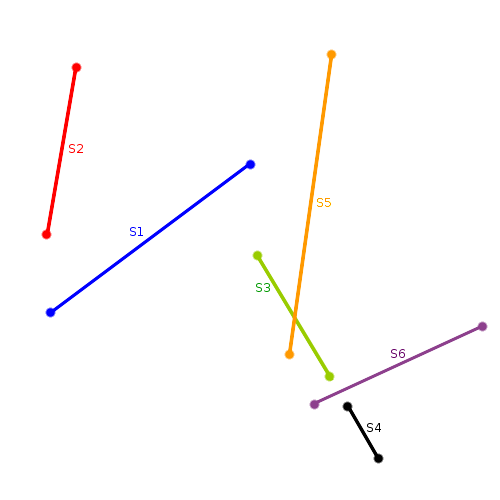
\includegraphics[scale=0.6]{bsp_ex_1.png}
\caption{Scène 2D}
\label{scene_inordre}
\end{figure}

Nous pouvons remarquer que cette scène contient 6 segments distincts, dont deux (les segments S3 et S4) se situant sur une même droite. Nous avons également des segments qui s'intersectent, ce qui va inexorablement mener à la création de nouveaux segments. Nous allons maintenant appliquer et expliquer le fonctionnement de l'heuristique "inordre", celui-ci étant représenté dans le plan à la Figure \ref{bsp_inordre} et l'arbre BSP correspondant est construit à la Figure \ref{bsp_tree}. \\

Cette heuristique travaille avec la liste des segments telle qu'elle a été fournie par l'utilisateur, c'est à dire que la création de l'arbre se fait dans l'ordre par lequel les segments ont été définis. \\

Nous commençons donc par une division du plan à l'aide de S1, et nous remarquons d'ores et déjà que S5 est alors coupé en deux segments S5A et S5B, en effet S5 intersecte la droite issue du prolongement de S1. Nous obtenons donc maintenant deux sous-ensembles de segments : 
$$S1^+ = \{S2, S5A\}$$
$$S1^- = \{S3,S4,S5B,S6\}$$
Récursivement, l'algorithme va être appelé sur $S1^+$ et $S1^-$. Et c'est le premier segment de la liste qui sera utilisé comme nouvelle droite définissant les nouveaux plans. 
\begin{itemize}
\item Pour $S1^+$ on a donc ainsi $S2$ comme segment de base pour la nouvelle droite. Il ne restera ainsi plus que $S5A$ comme feuille. 
\item Pour $S1^-$ on a $S3$ comme origine de la nouvelle droite et on remarque que $S4$ est également inclu à la droite, donc ces deux segments font alors partie du même noeud. Nous avons également que $S3$ intersecte $S5B$ et $S6$ ce qui engendre la création des segments : $S5C$, $S6A$, $S6B$, la suppression du segment $S6$ et la modification de $S5B$ (qui se traduira néanmoins techniquement par la suppression et la création d'un segment avec les coordonnées mises à jour). 
\end{itemize}

\begin{figure}[!h]
\centering
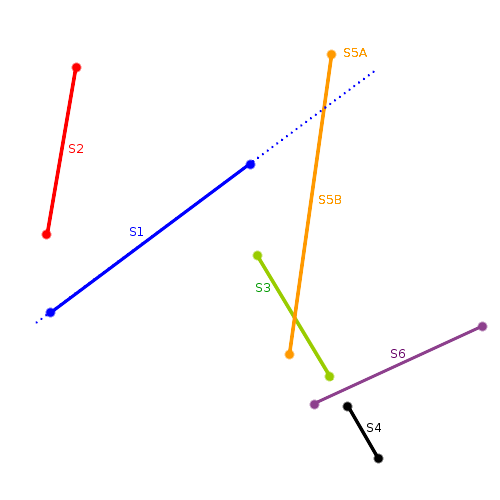
\includegraphics[scale=0.6]{bsp_ex_2.png}
\caption{Application de l'heuristique}
\label{bsp_inordre}
\end{figure}

\begin{figure}[!h]
\centering
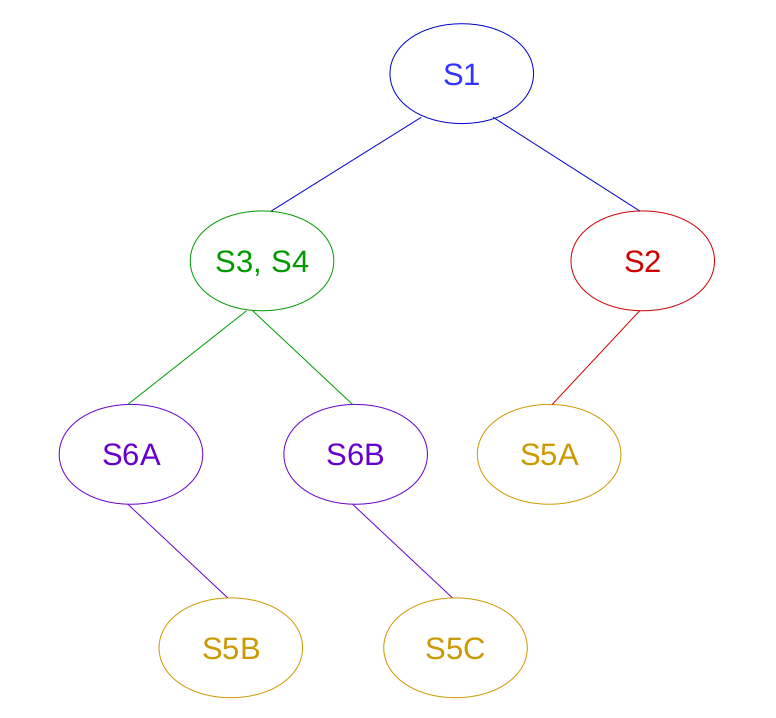
\includegraphics[scale=0.35]{bsp_ex_3.png}
\caption{Arbre BSP}
\label{bsp_tree}
\end{figure}

\paragraph{Implémentation \& Complexité}

\subsubsection{Heuristique "random"}

Cette heuristique utilise la même méthode que l'heuristique "inordre" pour la création de l'arbre BSP, à la seule différence près que la liste des segments est mélangée avant de commencer la construction. La différence d'un point de vue algorithmique avec l'heuristique précédente étant nulle, nous ne attardons donc pas sur ce point. 

\subsubsection{Heuristique "free-splits"}

\paragraph{Méthode}

Afin d'expliquer au mieux cette heuristique, nous utiliserons également un exemple, représenté à la Figure \ref{scene_splits}. \\

Cette heuristique se veut plus réfléchie que la simple utilisation, dans un ordre aléatoire ou non, des segments pour la définition de nouveaux plans. Nous allons donc étudier ici le cas particulier des "free-splits", ce dernier n'apparaissant que dans des circonstances bien précises, recréées ici dans l'exemple. Notons que cette heuristique se base sur une liste de segments ordonnés de manière aléatoire, néanmoins, pour les besoins de l'exemple nous supposerons que l'algorithme traite les segments dans l'ordre où ceux-ci ont été définis. En effet, si nous traitons les segments dans un ordre aléatoire, il se pourrait que nous soyons en présence d'une situation ne disposant pas de "free-split".

\begin{figure}[!h]
\centering
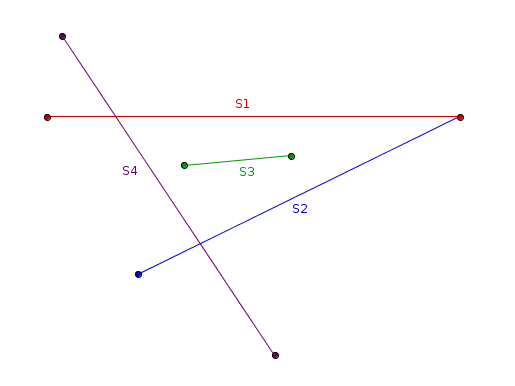
\includegraphics[scale=0.5]{free_splits_2.png}
\caption{Scène 2D}
\label{scene_splits}
\end{figure}

Exécutons pas à pas l'algorithme et définissons à l'aide de l'exemple la notion de "free-split". \\

Nous pouvons observer que cette scène est composée de 4 segments. Imaginons que nous avons déjà construit une partie de l'arbre BSP avec S1 et S2, nous remarquons alors que ces deux segments coupent S4, ce qui divise S4 en trois nouveaux segments (nommés S4A, S4B et S4C dans la Figure \ref{heuristic_splits}). A cette étape nous avons déjà la partie gauche de l'arbre construite avec S4A en tant que feuille (voir Figure \ref{split_bsp}). Il reste alors à construire le côté droit à partir de S2. S4C étant tout seul de son côté, le choix se porte alors entre S3 et S4B comme base pour une nouvelle droite. Or étant donné que S4B est déjà intersecté par deux droites, l'utiliser comme nouvelle droite ne causera pas de nouvelle fragmentation lors de la création du noeud ! C'est ce que l'on appelle la notion de "free-splits", c'est à dire utiliser des segments déjà intersectés par deux droites existantes pour définir de nouveaux plans, car ceux-ci, par conséquent ne fragmenteront plus aucun segment. Ce qui est avantageux tant au niveau du temps d'exécution de l'algorithme et qu'au niveau de la quantité de segments qui est alors réduite.\\

Notons que lorsqu'aucun "free-split" n'est présent, c'est l'algorithme "random" de création d'arbre BSP qui est d'application. 

\begin{figure}[!h]
\centering
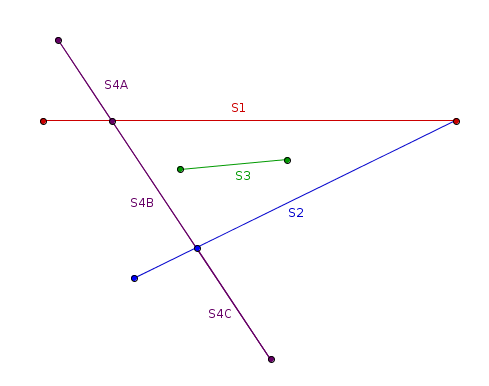
\includegraphics[scale=0.5]{free_splits_1.png}
\caption{Application de l'heuristique}
\label{heuristic_splits}
\end{figure}


\begin{figure}[!h]
\centering
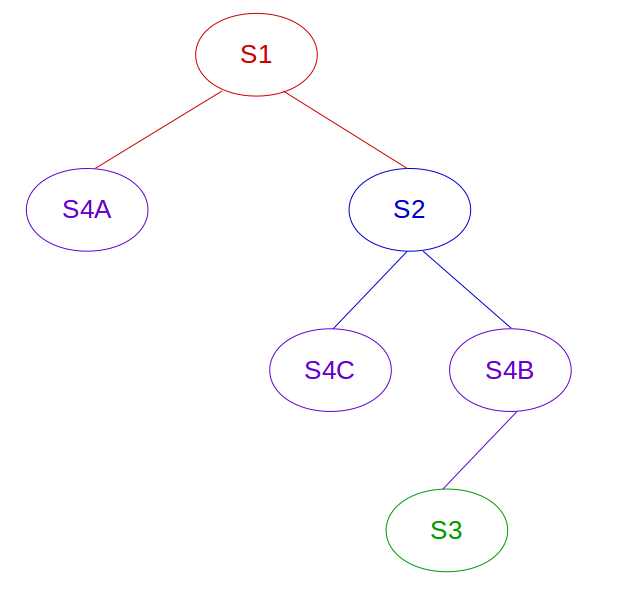
\includegraphics[scale=0.4]{free_splits_3.png}
\caption{Arbre BSP}
\label{split_bsp}
\end{figure}

\paragraph{Implémentation \& Complexité}

\subsection{Tests \& Résultats}

\section{Algorithme du peintre}

\subsection{Détails sur l'algorithme}

\subsection{Implémentation}

\subsection{Tests \& Résultats}

\section{Interface graphique}

%TODO : Expliquer les subtilités de l'utilisation ? 

\section*{Conclusion}
\addcontentsline{toc}{section}{Conclusion}
\end{document}